\documentclass[11pt]{article}
\usepackage{braket}
\usepackage{enumitem}
\usepackage{latexsym}
\usepackage{amsfonts}
\usepackage{amsmath,amssymb,amsthm}
\usepackage{xcolor}
\usepackage{mathrsfs}
\usepackage{tikz}
\usetikzlibrary{arrows}
\usetikzlibrary{automata}

\setlength{\textheight}{8.5in}
\setlength{\textwidth}{6.0in}
\setlength{\headheight}{0in}
\addtolength{\topmargin}{-.5in}
\addtolength{\oddsidemargin}{-.5in}

\input{../lecture_notes/preamble.tex}

\newcommand{\solution}[1]{\paragraph{Solution}  }
\newcommand{\bl}[1]{\textcolor{blue}{#1}}
\newcommand{\rd}[1]{\textcolor{red}{#1}}

\begin{document}
\hw{5: Undecidability}{3/17/2023}{Rishav Bhagat}{Due:4/03/2023}

You should submit a typeset or \emph{neatly} written pdf on Gradescope.  The grading TA should not have to struggle to read what you've written; if your handwriting is hard to decipher, you will be asked to typeset your future assignments. Five bonus points if you use \LaTeX, and our template. You may collaborate with other students, but any written work should be your own. \textbf{This homework tests your proof writing skills. Grading will be done on your ability to articulate and form a technical argument.}

\begin{enumerate}
    \item Prove that $\{\braket{M} ~|~ 1001 \in L(M) ~\}$ is undecidable using the method of reduction.

    \solution{} Let $L_{1001} = \{\braket{M} ~|~ 1001 \in L(M) ~\}$ be the language in question. For contradiction, assume that $L_{1001}$ is decidable; that is, there exists a decider $D$ that decides this language (it halts on all inputs). Using this decider, we can build a decider $S$ for $A_{TM} = \{\braket{M, w} ~|~ M \text{ accepts } w\}$, which is a language known to be undecidable. We build $S$ as follows:

    \begin{verbatim}
        S on <M, w>:
            build M'(x) so M' first simulates M on w. Then if M accepts,
                M' should accept its input x. If M loops forever, M'
                will loop forever on x. If M rejects, M' rejects x.
            If L(M') contains 1001 (checked through the decider D):
                accept
            else:
                reject
    \end{verbatim}

    Note that we never actually run $M'$, which may or may not halt, so $S$ will always halt since $D$ always halts. Also note that if $1001 \in L(M')$, that means that $M$ accepts $w$ since that is the only way $M'$ accepts any inputs. Thus, $S$ decides $A_{TM}$, which should not have a decider. This is our contradiction, so $L_{1001}$ must be undecidable.

    Another way of putting this is that $A_{TM} \leq_M L_{1001}$, $A_{TM}$ can be reduced into $L_{1001}$, so if $A_{TM}$ is undecidable, so is $L_{1001}$.
    
    \item Consider the function \begin{align}
        f(x) = \begin{cases}3x+1 & x\text{ is odd}\\x/2&x\text{ is even}\end{cases}
    \end{align}
    We use the notation $f^i(x)$ to represent repeated application of $f$ to $x$ an $i$ number of times. For example, $f^3(x) = f(f(f(x)))$. The Collatz Conjecture states $$\forall x \exists i [f^i(x) = 1]$$ with $x,i \in \mathbb{N}_{\geq 1}$. That is, repeated application of this function to any number will eventually reach 1. For example, if $x=17$, we get the sequence $$17,52,26,13,40,20,10,5,16,8,4,2,1$$ The conjecture remains a massive open problem in mathematics. It has been computationally verified for the first few million numbers, but has not been proven for all numbers. Consider the language $HALTALL = \{\braket{M}~|~ M \text{ halts on ALL inputs }\}$. It is obviously undecidable for similar reasons to $HALT$ and $A_{TM}$. Suppose you were given a decider for $HALTALL$ called $H$. Describe a method in which you could prove that the conjecture is either true or false.

    \solution{} First, note that $f$ is a computable function. This is obvious since we can easily write python code for it. Further, it is a composite of multiple turing computable operations (multiplication, division, addition, checking if a number is even or odd).

    Now, we build a turing machine $M$ as follows that takes in $x \in \mathbb{N}_{\geq 1}$:

    \begin{verbatim}
        M on x:
            1.  Run f on the tape
            2.  If the number 1 is the only thing on the tape:
                    accept x
                else:
                    go back to step 1
    \end{verbatim}

    Basically, $M$ will accept $x$ if $\exists i [f^i(x) = 1]$ and will otherwise loop forever and never halt, going through the sequence:
    $$ f^0(x),f^1(x),f^2(x),f^3(x),\dots, $$

    Now, using our decider $H$ for $HALTALL =  \{\braket{M}~|~ M \text{ halts on ALL inputs }\}$, we can run $HALTALL$ on $M$, which must either accept or reject (since it is a decider and must halt on all inputs).

    If $HALTALL$ accepts $M$, that means that $M$ halts on all inputs $x \in \mathbb{N}_{\geq 1}$, which means that $\forall x \in \mathbb{N}_{\geq 1} \exists i \in \mathbb{N}_{\geq 1} s.t. [f^i(x) = 1]$. This would prove the conjecture true.

    However, if $HALTALL$ rejects $M$, it would mean $\exists x \in \mathbb{N}_{\geq 1} \forall i \in \mathbb{N}_{\geq 1} s.t. [f^i(x) \neq 1]$, proving the conjecture false.
    
    \item This question tests your ability to apply the Church-Turing Thesis. See the attached chart on canvas. There are two axii. One of logical purism, neutrality, and rebellion. The other of existential purism, neutrality, and rebellion. I have provided an example for each of the nine categories, organized into a three by three table. Write a rigorous and persuasive argument as to which of the nine categories you can best apply the Church-Turing Thesis. Note you are not arguing correctness of the provided example, but of its category. Your argument should convince me your selection of the nine is correct, and the other eight are incorrect.

    \begin{figure}
        \centering
        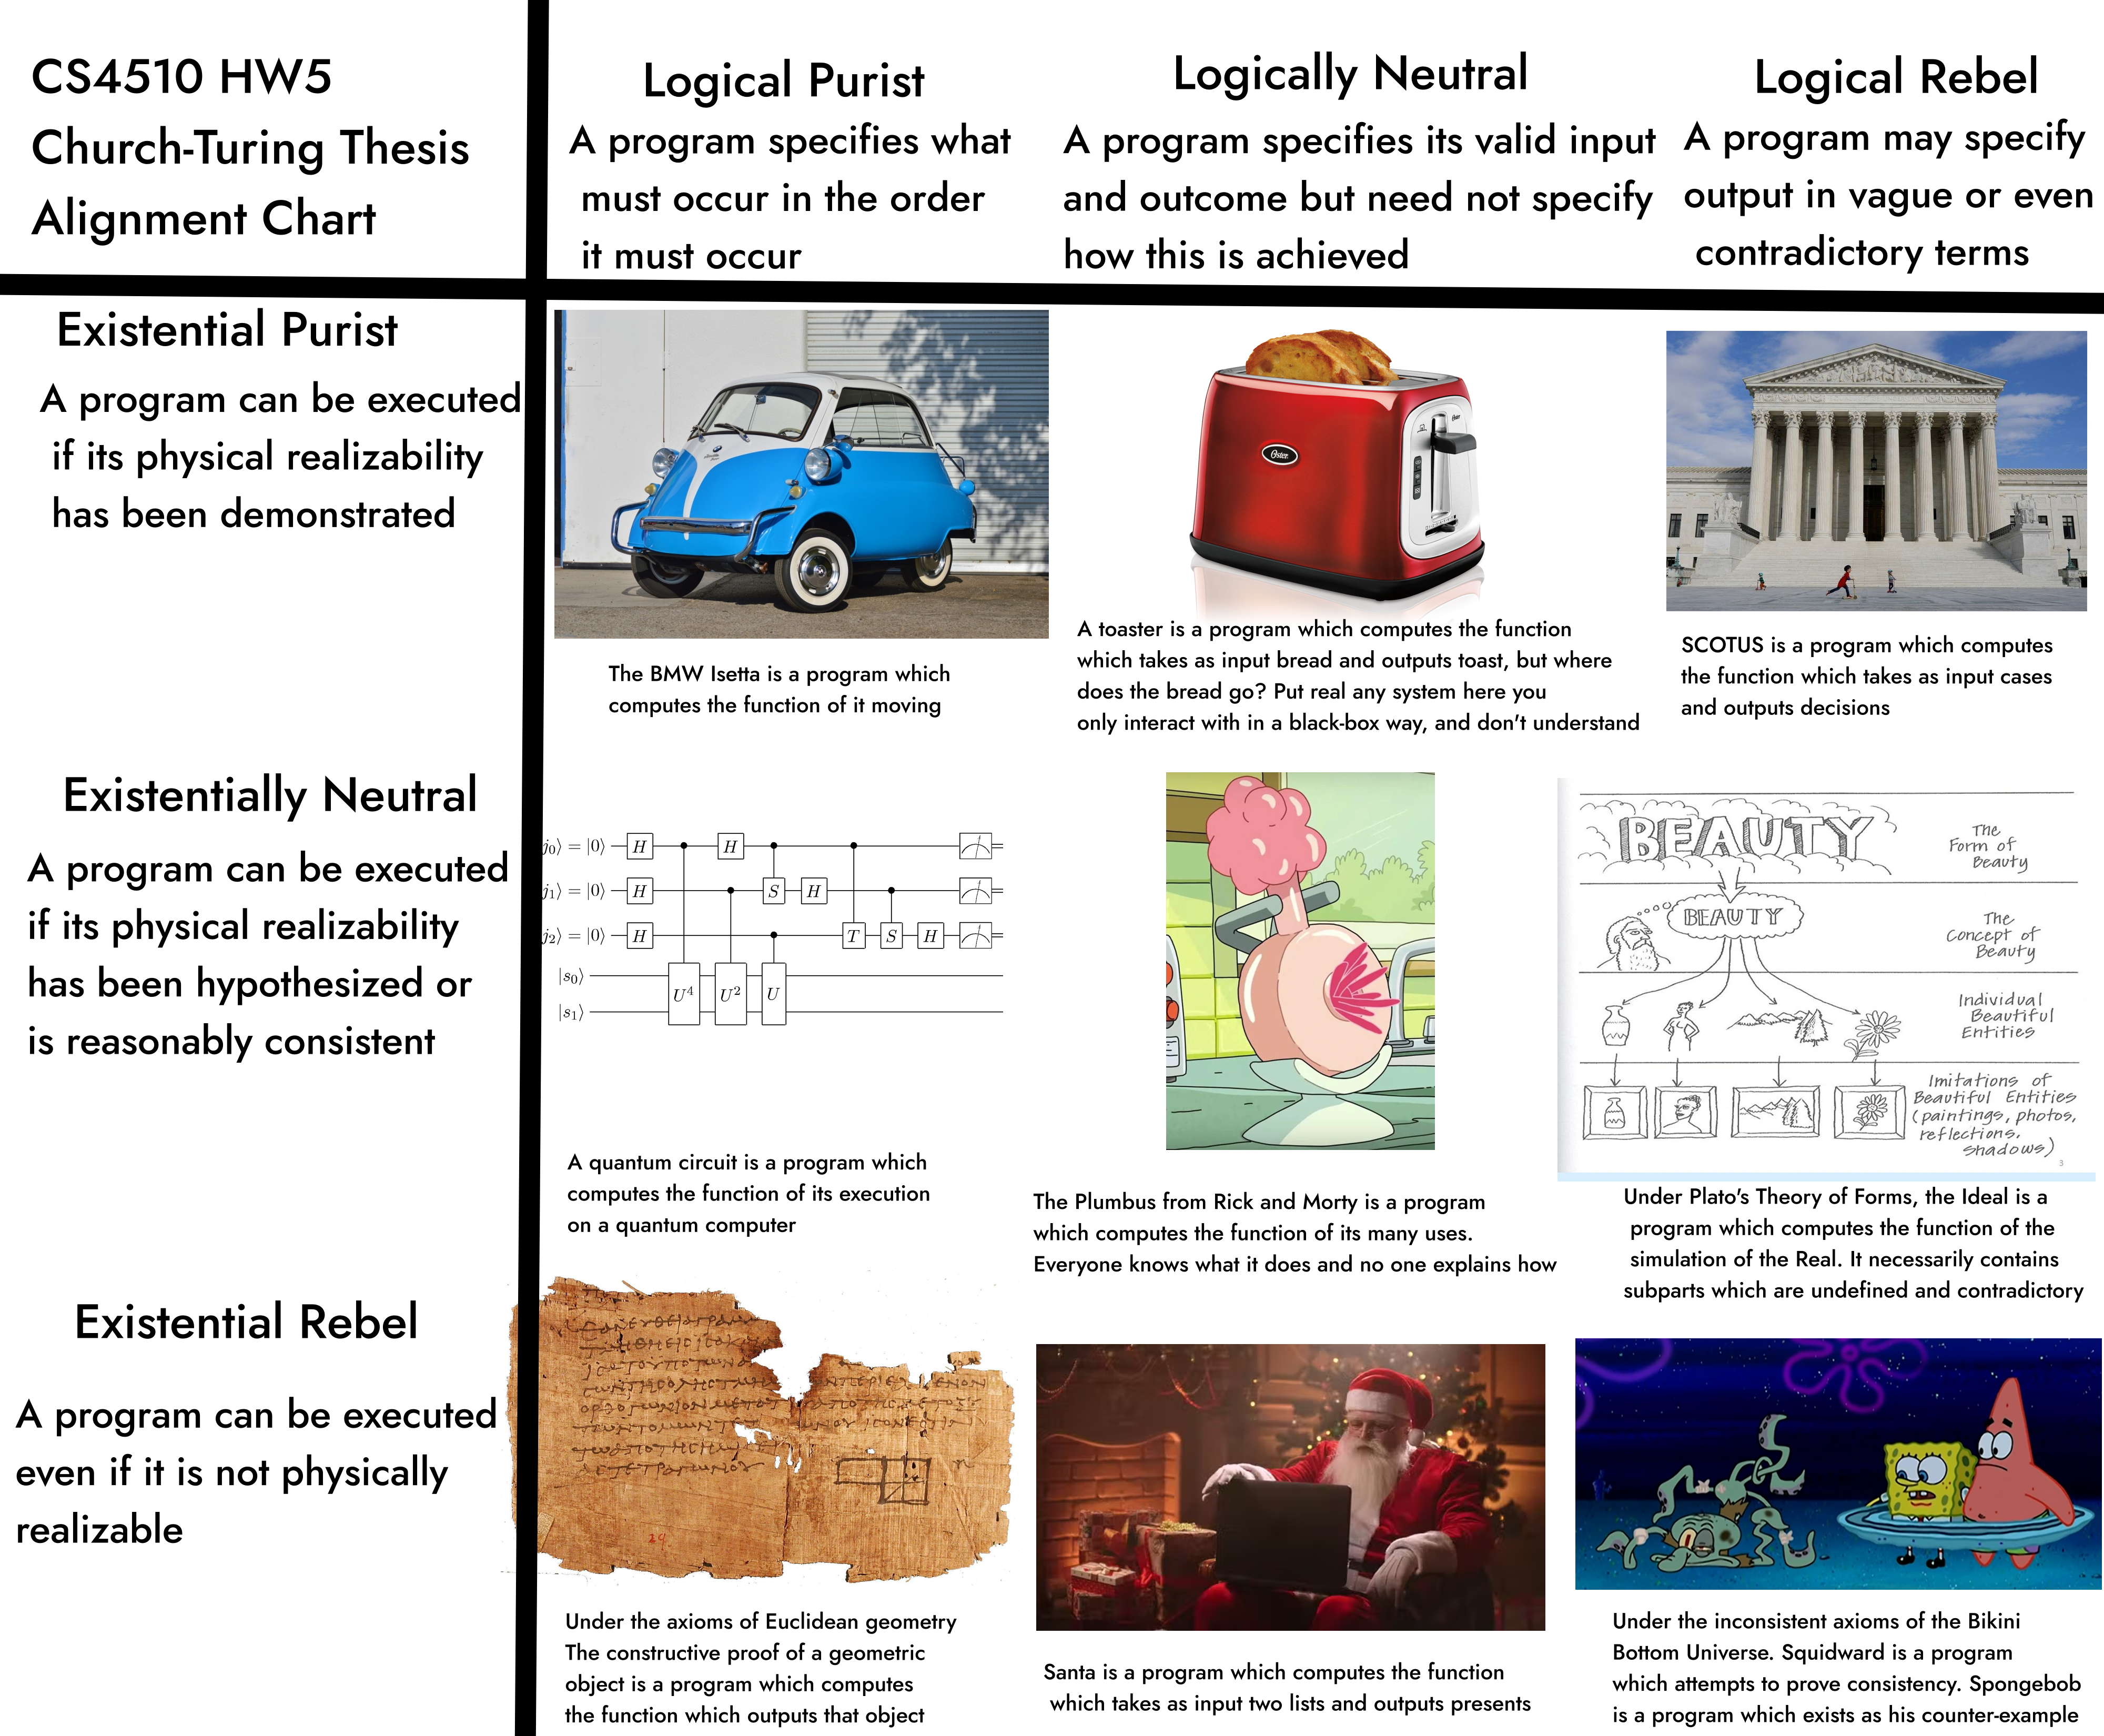
\includegraphics[width=\textwidth]{HW5/res/alignmentchart.png}
        \caption{Church-Turing Alignment Chart}
        \label{fig:my_label}
    \end{figure}

    \solution{} The Church-Turing Thesis follows \textbf{logical purism} since it states that Turing Machines are as powerful as anything we can create is and they specify what must occur in the order it must occur to get to a certain output. A Turing Machine does not work as a black box like specified in logically neutral and does not specify a vague or contradictory terms like a logical rebel machine either.

    The Church-Turing Thesis follows \textbf{existential neutral} as well since Turing Machines are hypothesized physical realizable in many ways. Many turing machines have not been demonstrated to be physically realized, but they can still be hypothesized and simulated (either through a universal turing machine or other simulators). Turing Machines are physically realizable and by the Church Turing thesis are as powerful as we can create, so we cannot execute a program that is not physically realizable as stated in existential rebel.
    
    \end{enumerate}

\end{document}
